\chapter{Design, Methodology \& Implementation}
This chapter ties the material from the previous chapter to this project by outlining its design, technique, and execution, as well as the rationale behind the choices made along its course.

\section{General Design and Methodology} \label{Design:GeneralDesign}
Current heuristic-based approaches for identifying function pairs suitable for merging, often miss opportunities for optimisation. This project aims to improve compiler function merging by leveraging machine learning to predict function pairs likely to produce beneficial merges.

For this approach to succeed, comprehensive training data consisting of diverse function pairs and their merging performance must be collected. These functions will be encoded into vector representations using IR2Vec to quantify their semantic meaning. The collected data will be processed to normalise before being used to develop, train and evaluate different ML models. To train the neural network architectures, the model will be fed labelled function pairs consisting of the function's vector representation and the merging performance. Once trained, this model, which predicts alignment scores for new function pairs, will be integrated into F3M to improve the function selection decisions.

The project methodology is structured around three interconnected stages: data collection, machine learning model development, and integrating everything, shown visually by figure \ref{fig:ProjectPipeline}.

\begin{figure}[tbh!]
\centering
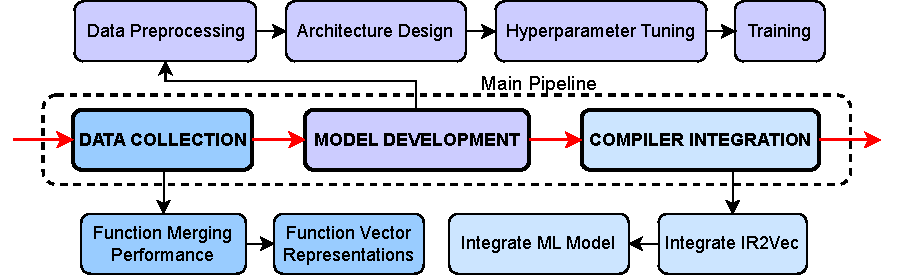
\includegraphics[scale=1]{Figures/ProjectPipeline.drawio.pdf}
\caption{End-to-end pipeline: From data collection of merging performance, through ML model development and evaluation, to final component integration to produce a working function merging pass.}\label{fig:ProjectPipeline}
\end{figure}

The first stage involves collecting a diverse dataset of merging performances to train the neural networks. This involves gathering two essential components: a suitable vector encoding of functions that captures their semantics and a metric that quantifies the similarity between function pairs to determine whether merging would be beneficial.

In the second stage, various machine learning architectures are explored and fine-tuned using the collected data to evaluate their performance in predicting merge suitability. This experimentation allows us to identify the most effective model architecture for function merging.

In the final stage, the trained models and function encodings are integrated into the LLVM compiler and evaluated on a suite of benchmarks to measure their overall code size reduction performance.

This project also includes artifacts for reproducing results, including a setup script, which will be detailed in the subsequent sections, along with elaborations on each stage of this process, providing insight into the design decisions and implementation details.

\section{Data Collection} \label{Design:DataCollection}
For this project, we gather vector representations of individual functions and pairwise functions' alignment scores, as defined in Section \ref{METRIC:AlignmentScore}. Since machine learning models perform better with numerical data than raw text, we encode function semantics using IR2Vec (Section \ref{subsubsec:IR2Vec}). IR2Vec operates directly on LLVM IR and, being open source, can be customised to our needs.

Next, the F3M codebase was extended to interface with a database, storing each function pair's merging performance and outcomes. To create a diverse dataset, we use a representative set of benchmarks that are commonly used in this research area, cc1plus, Chrome, LibreOffice, Linux, LLVM, SPEC2006, and SPEC2007, provided as bitcode files in F3M's artifacts. F3M's function merging mechanism was applied to every possible function pair across these benchmarks to collect their merging performance. While F3M computes multiple metrics, the alignment score was selected as the primary measure as it effectively captures the structural similarity between functions and is important for merging decisions.

Since two sources are used for data collection, a good database design is needed to relate and efficiently store the data accurately.

\subsection{Use of IR2Vec} \label{subsection:UseOfIR2Vec}
\textbf{\textit{IR2Vec}} (Section \ref{subsubsec:IR2Vec}) was employed to transform the IR of each function into a 300-dimensional vector embedding. This wide dimensionality allows the encoder to capture more detail for each function. This process also produces an embedding for every function, making it a perfect fit for our needs to work at function-level granularity. Additionally, IR2Vec was selected because of its proven ability to capture both the semantic meaning and flow of LLVM IR.\cite{IR2Vec}. Its efficient encoding process and graceful handling of out-of-vocabulary tokens via seed embedding vocabulary further contribute to its appeal as an encoder. 



\subsection{Database Solution}
Before collecting any data, it was necessary to determine a suitable storage solution that fits the project's needs.

\paragraph{SQL} \textbf{\textit{SQL}} databases offer significant advantages over other file structures like \textit{CSVs} and \textit{Pandas} primarily due to the expressive power of the SQL query language. Rather than reinventing the wheel each time a complex query is required, SQL provides users with a rich set of built-in functions and operators. This expressiveness simplifies the querying and enhances performance, especially when working with large volumes of data, by leveraging optimised indexing and storage mechanisms. In contrast, Pandas loads the entire dataset into memory, making it impractical for extremely large datasets like we will have. Furthermore, the relational nature of SQL databases, where data is organised into interconnected tables, enables more efficient modifications and queries across related data sets, reducing redundancy and improving maintainability.

\paragraph{SQLite} \textbf{\textit{SQLite}} was selected over other SQL solutions, such as \textit{PostgreSQL}, primarily for its ease of use and minimal configuration requirements. Unlike PostgreSQL, which typically requires extensive setup, including robust security configurations and server management, SQLite operates as a server-less, file-based database, making it an ideal choice where sensitive data is not a concern. This centralised-file design also simplifies creating a portable artifact, which was a prime consideration in providing a replicable project. Additionally, SQLite provides a C++ interface, the language used to build LLVM and F3M. Finally, its widespread adoption in the Python ecosystem offers an advantage, popular libraries like \textbf{\textit{Pandas}} and \textbf{\textit{TensorFlow}} provide support to read data from SQLite directly, enabling straightforward connections and interactions.

\subsection{Database Design} \label{subsection:DatabaseSchema}
The design of this database schema is guided by the need to efficiently store and query data, especially since the number of function pairs scales quadratically to the number of functions in a program.

\begin{figure}[tbh!]
\centering
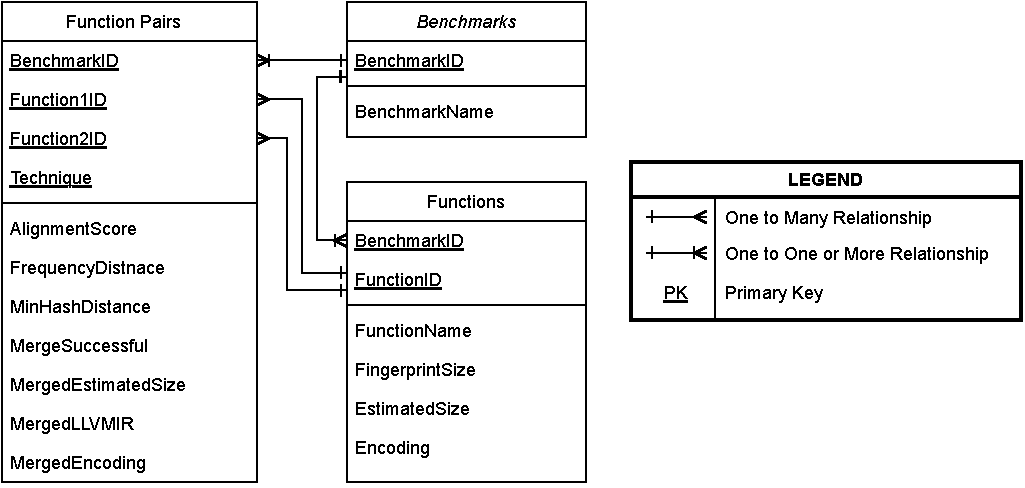
\includegraphics[scale=0.85]{Figures/DataCollectionSchema.pdf}
\caption{Schema of database used to store collected data using crows foot notation}\label{fig:DatabaseSchema}
\end{figure}


The schema consists of three primary tables, as Figure \ref{fig:DatabaseSchema} illustrates. The \textbf{Benchmarks} table serves as the top-level reference point for all data points. This design ensures that each evaluated dataset is logically isolated, facilitating independent analyses and debugging if needed.

The \textbf{Functions} table captures detailed information about individual functions for each benchmark. Combining \textit{BenchmarkID} and \textit{FunctionID} as composite keys ensures that function identifiers are scoped locally within each benchmark, preventing cross-function ID collisions. The foreign keys ensure that each function entry is associated with a valid benchmark.

Each function's name is recorded as a unique key for linking F3M outputs to IR2Vec embeddings. The fingerprint size is computed as the sum of the frequencies of opcodes in HyFM's function fingerprints. Function size is then estimated by summing LLVM's per‑instruction code‑size costs, queried via the TargetTransformInfo interface.

The functions' encodings are stored as BLOB type to store a pickled Python list representing the function's vector encoding. This decision aims to reduce redundant data transformations since the encodings are generated and used in Python (during training). Storing them directly in binary format avoids unnecessary conversions to and from string representations.

Finally, the \textbf{FunctionPairs} table stores all function pair comparisons. The foreign keys ensure that referenced benchmarks and functions exist. This table only uses a single BenchmarkID alongside two function IDs because function merging is only performed within the same program. This table also stores the distance metrics, AlignmentScore (\ref{METRIC:AlignmentScore}), the pairwise fingerprint distance computed by HyFM \cite{HyFM:FunctionMergingForFree}, the pairwise fingerprint distance computed by F3M and any merging outcomes.

\subsection{Data Collection Framework}
The data collection step was split into two steps, one to collect information on F3M's merging attempts and one to collect the functions' embeddings from IR2Vec.

An automated scripts were made for each step, both sharing many similarities. The user would specify a base directory of the benchmarks, and the script would dive into the directory and sub-directories, looking for any benchmark's bitcode files. 
The scripts have additional parameters to specify the database's stored name and file path, ensuring that different runs do not interact with the same default database. This allows multiple shell sessions to run the same script concurrently on different benchmarks, enabling several benchmark data collections to occur simultaneously. This concurrent execution saves time since each script processes benchmarks sequentially and prevents the corruption of the SQLite file, as SQLite does not do concurrency very well.

\subsubsection{Collecting F3M Merging Metrics}
Merging metrics are collected before function encodings since not all functions touched on IR2Vec would be merged in F3M, decreasing the amount of functions' vector representations to collect.

F3M provides a reporting feature that outputs the computed metrics for every function pair's merging performance. To collect merging metrics, F3M's implementation within the LLVM codebase is repurposed to use SQLite's C++ interface, piping the pairwise metrics directly into the database instead of the terminal or log files. This approach simplifies the implementation and decreases data collection time by eliminating any post-processing of log files. After these changes, LLVM's optimiser is run on the bitcode files, invoking the F3M pass with the reporting flag to collect all pairwise data.

After running the scripts from this step, all fields in the new database should be populated except for the encoding field, which will be populated in the next step.

\subsubsection{Collecting IR2Vec Function Encodings}
Function encodings are collected separately because each function is encoded only once while merging metrics are computed for every function pair.

IR2Vec's binary was used to generate function-level embeddings from the bitcode files with flow-aware embeddings to better capture the relational aspects between the components in the file. A compatibility issue was identified with IR2Vec. The function names used by IR2Vec and LLVM are different. LLVM's function retrieval returns mangled function names, while IR2Vec produces demangled names. Consequently, IR2Vec's source code was modified and rebuilt to conform to LLVM's naming convention. 

The encodings are output and stored in text files, a medium provided by IR2Vec. An assistive script is then made to load the encodings from the text files into the database as a serialised binary object. After connecting to the database, the script retrieves the corresponding database entry after accessing it and updates it with the embedding. 

\subsubsection{Merging Data}
Since multiple scripts were run concurrently while writing to different databases, a script was created to merge all data into a single, centralised database automatically. The script accepts a variable number of arguments specifying the input databases to combine and an argument for the new database's name. It works by initialising a new database using the specified name, connecting it to each existing database, and then copying over the information.

\section{Model Development} \label{Design:ModelDevelopment}
To develop machine learning models, the data from the previous step are pre-processed and partitioned to form a representative dataset. Then, two ML model architectures were designed, and a framework was established to support efficient training, testing, fine-tuning, and evaluation of these models, streamlining experimentation and providing a reliable structure for iterative improvements.

\subsection{Data Pre-Processing}
\subsubsection{Data Imbalance} \label{Design:DataImbalance}
A major challenge encountered with the dataset was the overwhelming number of function pairs with an alignment score of 0. In total, there were \textbf{\textit{2.2 billion}} function pairs collected, of which \textbf{\textit{1.67 billion}} samples had an alignment score of 0 (zero-samples), \textbf{\textit{1.7 million}} had an alignment score of 1 (one-samples) and \textbf{\textit{570 million}} has an alignment score between 0 and 1 (non-zero-non-one samples). If this imbalance is not adequately addressed, the model would likely learn to predict 0 for most situations to achieve a superficially low error but produce unhelpful predictions.

This imbalance is mitigated in two ways. First, a large portion of the zero samples is discarded so that the remaining zero samples equal the combined total of one and non-zero-non-one samples.
$$Zero\ Samples = One\ Samples + Non\_Zero\_Non\_One\ Samples$$
This balancing strategy reduces the dominance of zero samples and decreases overall training time by lowering the total number of training examples. Secondly, during model training, each remaining zero-alignment sample is assigned a weight of \textbf{\textit{0.001}}. This weighting means that every non-zero alignment sample contributes 1,000 times as much to the loss function as a zero-alignment sample, thus diminishing the influence of the overly abundant zero samples. This way, the model is incentivised to learn accurate predictions for non-zero alignment scores.


\subsubsection{Data Split} \label{Design:DataSplit}
After collecting and processing the data, we end up with \textbf{\textit{1.1 billion}} function pairs. The order of data is then randomised to make it diverse when encountered by the machine learning model, preventing bias from improving generalisation and stopping the model from learning misleading patterns based on data sequence. After which, the dataset is split into three smaller SQLite datasets, the training, validation and testing datasets, each making up 70\%, 10\% and 20\% of the pre-processed dataset, respectively. The model uses the training dataset to train itself. In contrast, the model uses the validation set to tune its hyperparameters (discussed in section \ref{subsubsection:HyperparameterTuning}). The test set is then used to test the model's performance on unseen data.

Pre-splitting the dataset accelerates training by eliminating the need to determine the data split during runtime, an extremely time-consuming process when working with a very large dataset. Furthermore, maintaining a permanent split throughout the model development stage reduces uncertainty in performance evaluations, as the deterministic nature of the split ensures consistent results. Consequently, any changes in metrics could be mainly attributed to the model's performance.

\subsection{ML Model Design}
The machine learning model developed will take in two functions' embeddings as inputs and produce an alignment score as the output.

% The alignment score provides a robust distance metric for function merging by capturing the structural and semantic similarity between code sections, discussed in section \ref{METRIC:AlignmentScore}. Compared to fingerprint distances used by HyFM and F3M, the alignment score excels at detecting equivalent code regions, giving early and strong insight into the potential code size reduction achieved when merging a pair of functions and measuring how well the pair overlaps.

Two model architectures were designed to predict the alignment score. The first is a Siamese model that uses dot product to quantify the similarity between the function embeddings. The second model features an attention mechanism to prioritise different elements of the inputs when making its predictions. Both models share the same goal with different approaches, the former modifies the input to fit the purpose better while the latter picks the most important information from the input to make its prediction. Comparing these methods allows us to evaluate which is more effective at alignment-score prediction.

\subsubsection{Dot Product Siamese Model}
This is an implementation of the Siamese network discussed in section \ref{ML:SiameseNetwork}, which uses a shared encoder to process two function encodings and then compare them using a dot product similarity. Figure \ref{fig:SiameseModelDesign} visually shows the architecture design of the dot product Siamese model.

\begin{figure}[tbh!]
\centering
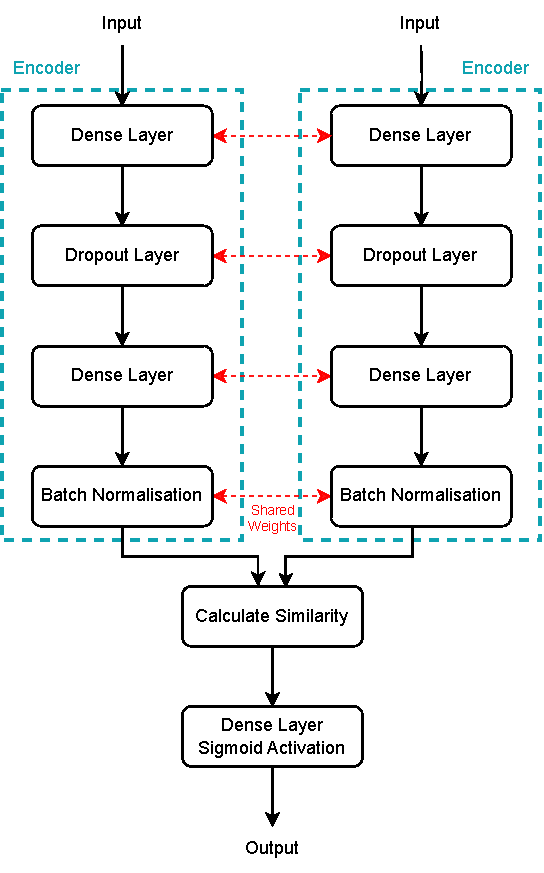
\includegraphics[scale=1]{Figures/SiameseModel.drawio.pdf}
\caption{\textbf{Visual representation of the Dot Product Siamese Model.} The encoders for both models share the same weights to map both functions' features onto the same function space. }\label{fig:SiameseModelDesign}
\end{figure}

\paragraph{Shared Encoder} The shared encoder projects IR2Vec's embeddings into a suitable feature space for comparison using the dot product. This works by clustering functions that merge well with each other in the feature space so the dot product can produce higher scores for embeddings that are close.

The shared encoder first expands IR2Vec's 300-dimensional vector in 512 dimensions to try and capture any more semantics lost due to the limited amount of elements, followed by a dropout layer with a dropout rate of 16.6\% to prevent overfitting. Then, a dense layer compresses the new 512 dimensions into 128 to abstract and retain the most relevant information for the comparison task.  

After this, batch normalisation is applied to standardise the layer outputs. This also reduces the need for careful initialisation and allows higher learning rates, effectively requiring one less hyperparameter to tune than a regular normalisation layer.

\paragraph{Score Generation}
Once both function embeddings have been processed through the shared encoder, the similarity between the embeddings is measured to capture how aligned the two functions are in the embedding space. Two similarity metrics, the dot product and cosine distance, are evaluated against each other to identify the most effective metric for this task. This similarity value is then passed through a dense layer of 1 unit with a sigmoid activation function to map the dot product to the [0,1] range, corresponding to the alignment score range.

\subsubsection{Multi-headed Self-Attention Model}
This is an implementation of a model which takes advantage of the attention mechanism discussed in section \ref{ML:AttentionMechanism}, visually shown by figure \ref{fig:AttentionModelDesign}.

\begin{figure}[tbh!]
\centering
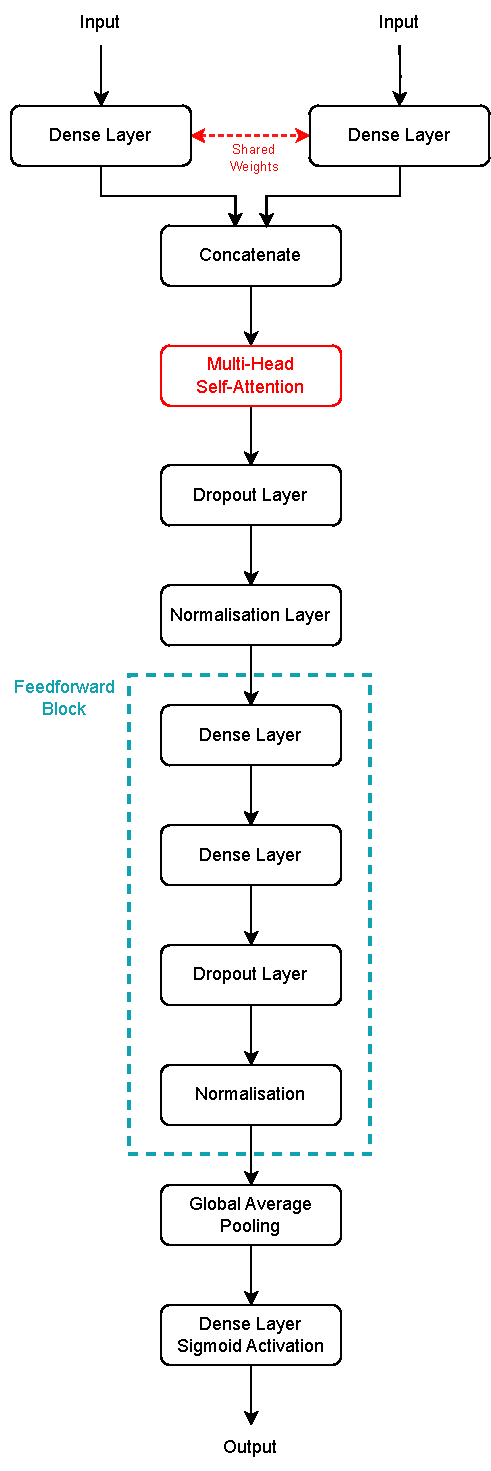
\includegraphics[scale=0.8]{Figures/AttentionModel.drawio.pdf}
\caption{\textbf{Visual representation of the Multi-Headed Self-Attention Model.} The model uses the attention mechanism to allow each element to attend to another. }\label{fig:AttentionModelDesign}
\end{figure}


The model first processes each IR2Vec embedding through a shared dense layer with 512 units and ReLU activation, expanding the representation to capture richer semantic information. Unlike the Siamese model, these expanded representations are then reshaped and concatenated, allowing the model to treat the function pair as a unified sequence.

The core of this architecture is the attention block, which implements multi-head self-attention with four attention heads, each with a dimension of 64. This mechanism allows each function representation to attend to the other, capturing complex relationships between their features. 

The self-attention output passes through dropout (30\%) to prevent overfitting and uses skip connections and layer normalisation to stabilise training. The subsequent feed-forward network with ReLU activation further processes these attention-weighted representations through a dimension of 64 before returning to the original dimension. After the transformer encoding, the model applies global average pooling to aggregate the sequence information into a single vector representation. This condensed representation is passed through a final dense layer with sigmoid activation to produce an alignment score in the $[0,1]$ range.

By leveraging attention mechanisms, this model can potentially capture more intricate relationships between function pairs, learning which aspects of functions are most relevant for aligning functions.


\subsection{Hyperparameter Tuning} \label{subsubsection:HyperparameterTuning}
% \subsubsection{Hyperparameter Tuning} \label{subsubsection:HyperparameterTuning}
Due to the sheer volume of training data available, tuning the hyperparameters using the entire training dataset would be computationally prohibitive. Therefore, the hyperparameter tuning stage uses a subset of \textbf{\textit{300 million}} training samples. Once the optimal hyperparameters are identified through this procedure, the model will be retrained on the full dataset comprising 1.1 billion training samples using these optimal settings.

For the hyperparameter optimisation, \textbf{\textit{Optuna}} is employed. Optuna is an efficient, automatic hyperparameter optimisation framework that utilises Bayesian optimisation methods to navigate the hyperparameter space. Each evaluation of a particular set of hyperparameters is referred to as a \emph{trial}. During each trial, the model is trained on the subset of data, and its performance is measured on the validation set, specifically the mean squared error. The results from numerous trials guide the search process, balancing the exploration of new configurations and exploitation of known good regions in the hyperparameter space, ultimately converging towards a model with the lowest mean squared error with the optimal settings.

\subsection{Framework/Pipeline for Model Development}
This section discusses the framework design and explains key design decisions.

\subsubsection{Serialising Data}
Initially, the models loaded data using Tensorflow's dataset interface, which acts as a lazy iterator for querying the SQLite dataset. Tensorflow's SQL dataset interface could not be used because the encodings, which were stored as BLOB objects, required depickling before being loaded into the model.

Direct querying of the SQLite dataset proved extremely slow. Therefore, a script to serialise the data into \textbf{\textit{NumPy}} arrays was created. This approach significantly reduced the required processing operations, resulting in a speedup of approximately \textbf{\textit{60\%}} in loading and processing times compared to SQL querying.

The serialisation utilises two two-dimensional \textit{NumPy} arrays: one to store function encodings and another to store alignment scores. Each unique tuple (BenchmarkID, FunctionID) is assigned a new unique function ID for the encodings array. These function IDs are stored with their respective encodings occupying the remaining columns. The second array stores alignment scores of function pairs using three columns: the first and second function's unique ID and the pair's alignment score.

The \textit{NumPy} arrays are saved to binary files for direct loading when needed, speeding up the process compared to loading and parsing data from a text file. While the number of functions is manageable, it pales in comparison to the number of function pairs. To prevent overloading the system's memory when loading the pairwise metrics due to its volume, the array is split into multiple binary files with a specified number of samples (chunk size) in each file so that each file remains small and manageable for loading.

Selecting an appropriate chunk size during serialisation is crucial, as excessively large values can cause system crashes or deadlocks. During the serialisation process, the script verifies that at least 20\% of system memory is available before retrieving the next data batch. If insufficient memory is available, the script sleeps until adequate memory becomes available. A potential deadlock can occur if the script holds data in memory, waiting to meet the size requirement, but lacks sufficient memory to retrieve the additional data needed to offload the current data into storage, freeing up memory.

\subsubsection{Loading Data}
This process utilises the TensorFlow dataset interface, where the dataloader first loads all function encodings into memory and then processes each chunk of pairwise metrics by replacing unique function IDs with their corresponding encodings.

This loading process was observed to be time-intensive. To address this performance bottleneck, the \textbf{\textit{concurrent}} Python library was used to load the next data chunk in a separate thread while the model trains on the currently available data. These loaded chunks are placed in a queue, which the dataloader lazily iterates through, significantly reducing the time the model spends waiting for data preparation between chunks and accelerating the training process.

The data loader is configured to process only one additional file concurrently, as processing more files simultaneously provides no performance benefit and consumes excessive system memory. This is particularly important since each fully expanded input contains 601 32-bit float values, around 2KB (\ref{Calculation:InputSize}).

To prevent system crashes due to memory exhaustion, the loader verifies that at least 20\% of system memory is available before loading and expanding each new data chunk. This memory management strategy ensures stable operation throughout the training cycle.

\subsubsection{Running the Model}
To streamline the model development process, a centralised script was developed that efficiently handles training and hyperparameter tuning across different model architectures. The main script accepts various command-line arguments to specify the model type, the operational mode (training or hyperparameter tuning), the location to save the trained models and, when in training mode, the specific model parameters.

For this modular approach to function effectively, each new model must implement two standard interface functions: $get\_model()$ and $HyperParameterTraining()$. The $get\_model()$ function provides the main script access to the model, while \\$HyperParameterTraining()$ encapsulates any model-specific hyperparameter optimisation requirements. This standardised interface eliminates redundant code and significantly simplifies working with different model designs.

A \textbf{\textit{Jupyter Notebook}} was created for model evaluation and result visualisation. This notebook tests trained models against the test dataset, calculates the mean squared error, and generates comparative plots of predicted versus true alignment scores to demonstrate model performance visually.

\section{System Integration} \label{Design:SystemIntegration}
This section describes how IR2Vec and the trained ML models were integrated into the F3M's codebase to leverage the ML models for function merging decisions.

\subsection{Integrating Tensorflow}
The initial integration strategy involved using \textbf{\textit{PyBind}} to load the trained TensorFlow models into the compiler. This approach was selected because one variant of the Siamese Model had been developed using the L1 distance metric instead of the dot product. Since this implementation required a custom layer not natively available in TensorFlow, PyBind appeared advantageous for running Python code, allowing custom layers to be used.

However, PyBind consistently crashed when attempting to load TensorFlow models. Given these limitations, \textit{TensorFlow's C++ API} was adopted as an alternative solution for loading the trained models. This decision required abandoning the L1 distance Siamese model due to the engineering work required to support its custom layer in the new integration approach.

\subsection{Integrating IR2Vec} \label{Design:IntegratingLLVM}
Next, since IR2Vec was developed in C++, the initial approach involved incorporating its header files and source code from the official \textit{GitHub} repository. However, while testing the project, errors occurred whenever the compiler attempted to request embeddings from IR2Vec. This compatibility issue likely stemmed from version differences between the LLVM versions used by each project. IR2Vec was based on LLVM 18.1.8 at the time of this project, while F3M used version 18.0.0, necessitating an alternative solution.

The adopted workaround involved pre-generating function encodings using IR2Vec's stand-alone executable for the benchmarks and storing them in text files. During compilation, the system would then parse these files and load the encodings into a map for quick encoding lookup of each function.

This integration approach imposed a significant limitation: newly generated merged functions could not be considered candidates for further merging, as it was impossible to obtain embeddings for these new functions during compile time. This constraint restricted the optimisation potential to a single pass of function merging.

\subsection{How it all fits together}
The function merging process begins when all candidates are placed into a priority queue. As each candidate is processed, it is removed from the queue for assessment. The queue prioritises functions with larger fingerprint sizes, giving them precedence over smaller ones. During assessment, the system predicts the alignment score between the current function and all other candidates in the queue. Merging is only attempted with the function that yields the highest predicted alignment score.

\paragraph{Thresholding Alignment Score} Even when the highest-scoring function pair is identified, merging only proceeds if the alignment score exceeds a predetermined threshold value. This threshold mechanism prevents wasting compilation resources on unprofitable merges when a function may be unsuitable for merging with other functions in the queue. Multiple thresholding values were tested during evaluation, including 0.4, 0.5, and 0.6, to determine the optimal balance between merge opportunities and compilation efficiency.

\section{Artifactory and Set up Script} \label{Design:ArtifactoryAndSetUp}
\subsection{Repository and Accessibility}
All code developed for this project is publicly available as artifact in a GitHub repository, linked in appendix \ref{Artifacts}. This repository contains the complete codebase, including models, data processing scripts, integration components, and evaluation tools. The repository is structured to facilitate easy navigation and understanding of the project's components, with clear documentation for each module.

\subsection{Automated Setup Script}
To enhance accessibility and reproducibility, a comprehensive setup script has been developed that automates the installation and configuration process. The script applies custom configurations to ensure compatibility between components and prepares the system for immediate experimentation. This automation significantly reduces the technical barriers to reproducing the research.

A detailed README file is included in the repository root, providing comprehensive guidance through the project setup process. The documentation clearly outlines the required dependencies and tested environments to ensure compatibility. It includes straightforward installation instructions that walk users through the cloning process and execution of the setup script.

The setup script intentionally excludes the complete installation of IR2Vec, instead only cloning the repository and applying necessary patches. This decision was made because IR2Vec requires a local build of LLVM as a prerequisite, requiring extensive disk space and compilation time.













